\section{The G\texorpdfstring{\MakeLowercase{raph}}{raph}MAE Approach}

In this section, we present the self-supervised masked graph autoencoder framework---\model---to learn graph representations without supervision based on graph neural networks (GNNs). 
We introduce the critical components that differ \model from previous attempts on designing graph autoencoders (GAEs). 
%We couple the introduction with 


\begin{figure*}[htbp]
    \centering
    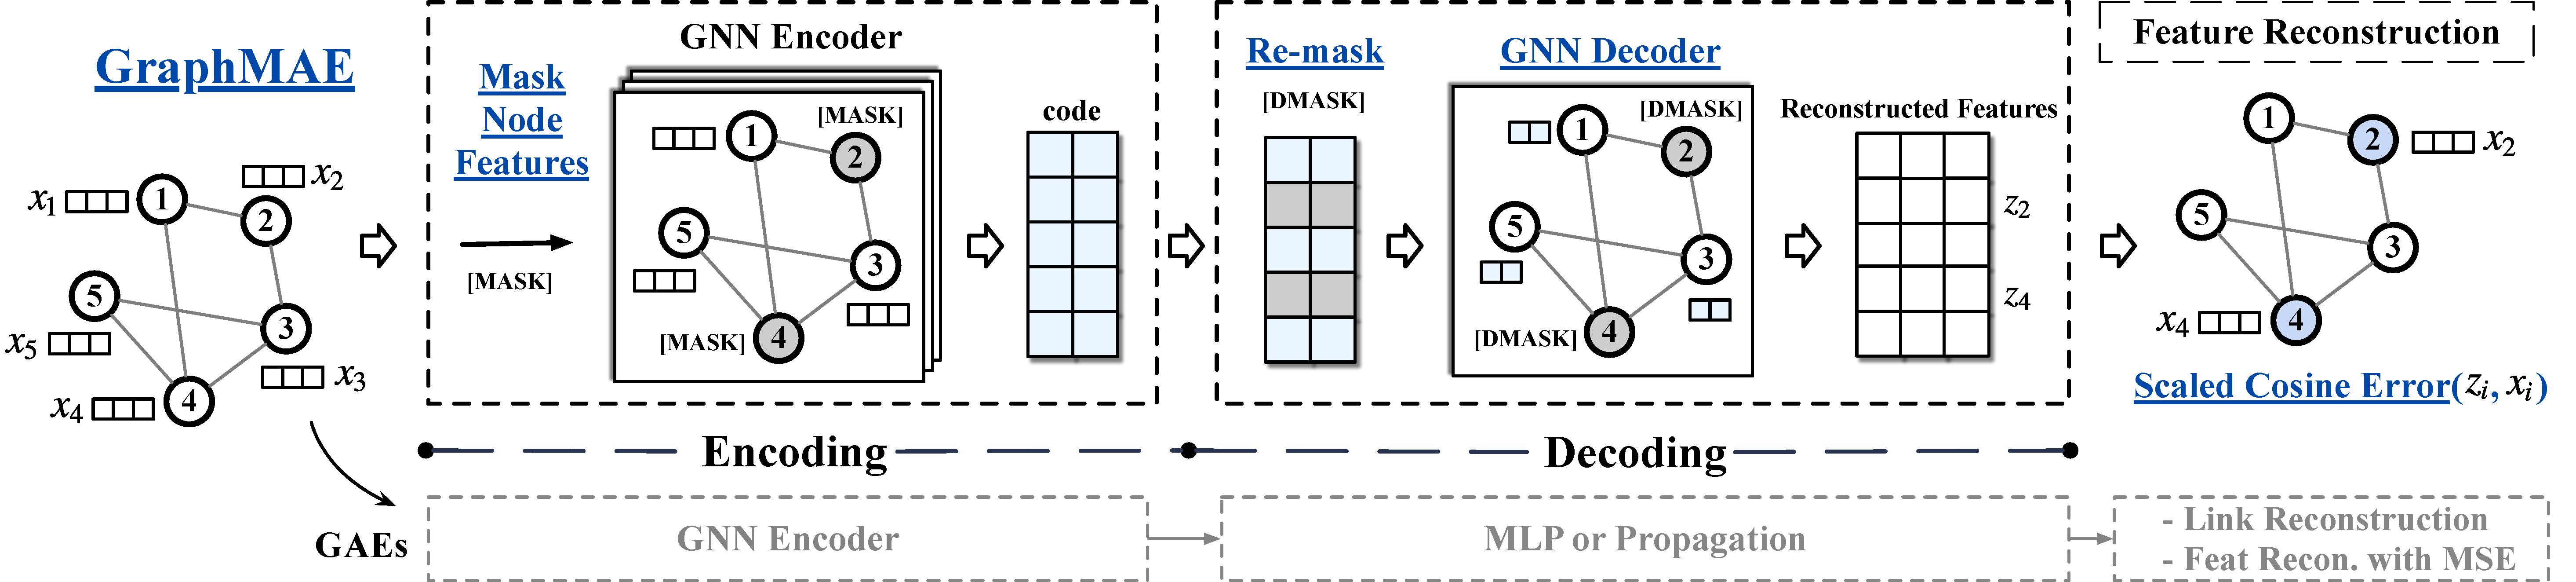
\includegraphics[width=\textwidth]{imgs/overview_sin.pdf}
    \caption{
    Illustration of \model and the comparison with GAE. 
    \textmd{We \underline{underline} the key operations in \model. 
    During pre-training,  \model first masks input node features with a mask token [MASK].  The corrupted graph is encoded into code by a GNN encoder. 
    In the decoding, \model re-masks the code of selected nodes with another token [DMASK], and then employs a GNN, e.g., GAT, GIN, as the decoder. 
    The output of the decoder is used to reconstruct input node features of masked nodes, with the {scaled cosine error} as the criterion.
    Previous GAEs usually use a single-layer MLP or Laplacian matrix in the decoding and focus more on restoring graph structure.}}
    \label{fig:overview}
\end{figure*}


\subsection{The GAE Problem and \model}

Briefly, an autoencoder usually comprises an encoder, code (hidden states), and a decoder. %, has been popular in representation learning for decades. 
The encoder maps the input data to code, and the decoder maps the code to reconstruct the input under the supervision of a reconstruction criterion. 
%To acquire a compressed knowledge representation, autoencoders usually impose a bottleneck in their architecture by enforcing a smaller dimension in code than the input.
For graph autoencoders, they can be formalized as follows. 
%We formally introduce the concept of graph autoencoders (GAEs) in the context of graphs. 

Let $\mathcal{G}=(\mathcal{V}, \mA, \mX)$ denote a graph, where $\mathcal{V}$ is the node set, $N=|\mathcal{V}|$ is the number of nodes, $\mA \in \{0,1\}^{N\times N}$ is the adjacency matrix, and $\mX \in \mathbb{R}^{N\times d}$ is the input node feature matrix. 
Further, given $f_E$ as the graph encoder, 
$f_D$ as the graph decoder, 
and $\mH \in \mathbb{R}^{N\times d_h}$ denoting the code encoded by the encoder, 
the goal of general GAEs is to reconstruct the input as 
\begin{equation}
    \begin{split}
        \mH = f_E(\mA, \mX), \ \mathcal{G}^{\prime} = f_D(\mA, \mH),
    \end{split}
\end{equation}
where $\mathcal{G}^{\prime}$ denotes the reconstructed graph, which could be either reconstructed features or structures or both.  
%The backbones for $f_E$ and $f_D$ can be any type of graph neural networks (GNNs), such as GCN~\cite{thomas2017gcn}, GAT~\cite{petar2018gat}, or GIN~\cite{xu2019powerful}. 


Despite their versatile applications in NLP and CV, autoencoders' progress in graphs, especially for classification tasks, is relatively insignificant. 
To bridge the gap, in this work, we aim to identify and rectify the  deficiencies of existing GAE approaches, and subsequently present the \model---a masked graph autoencoder---to further the idea and design of GAEs and generative SSL in graphs. 


\vpara{GraphMAE.}
The overall architecture of \model is illustrated in Figure~\ref{fig:overview}. 
Its core idea lies in the reconstruction of masked node features. %---defined as $\widetilde{\mX}$.  \todo{}
% To have a robust reconstruction, we propose to use a scaled cosine error as the criterion. 
% In addition, we introduce a re-mask decoding strategy with GNNs, rather than the widely-used MLP decoder in GAEs, to empower \model.
And we introduce a re-mask decoding strategy with GNNs, rather than the widely-used MLP in GAEs, as the decoder to empower \model.
% Furthermore, 
To have a robust reconstruction, we also propose to use a scaled cosine error as the criterion. 
% to enable \model with capacity. 
Figure \ref{fig:cmp_tab} summarizes the technical differences between % the proposed 
\model and existing GAEs. 


In detail, the backbones for $f_E$ and $f_D$ can be any type of GNNs, such as GCN~\cite{thomas2017gcn}, GAT~\cite{petar2018gat}, or GIN~\cite{xu2019powerful}. 
As our encoder $f_E$ processes the whole graph $\mA$ with partially observed node features $\widetilde{\mX}$, resonating to the backbones in other generative SSL methods (e.g., BERT and MAE), 
\model prefers a 
more expressive GNN encoder on features for different tasks. 
% more expressive GNN encoder based on different graph learning tasks
% \qinkai{Not clear. "more expressive GNN encoder based on different graph learning tasks"?}
For instance, GAT is more expressive in node classification, and GIN provides a better inductive bias for graph-level applications (See Tables~\ref{tab:backbone} and ~\ref{tab:ablation}). 

 







\subsection{The   Design of \model}

%\qinkai{It would be better if the entire process of graphMAE can be presented by pseudo codes.}
In this part, we explore how to design a generative self-supervised graph pre-training framework 
%such that it can leverage lessons learned from existing GAE efforts
that can match and outperform state-of-the-art contrastive models. 
Specifically, we discuss different strategies via answering the following four questions: 
\begin{itemize}[leftmargin=*,itemsep=0pt,parsep=0.2em,topsep=0.3em,partopsep=0.3em]
    \item \textbf{Q1}: What to reconstruct in GAEs? %, particularly 
    %for node/graph classification?
%    ?
    \item \textbf{Q2}: How to train robust GAEs to avoid trivial solutions? 
    %\qinkai{It's not clear how robustness is guaranteed from the writing and the results. }
    \item \textbf{Q3}: How to arrange the decoder for GAEs?
    \item \textbf{Q4}: What error function to use for reconstruction?
\end{itemize}
These questions concern the designs of the reconstruction objective, robust learning, loss function, and model architecture in GAEs, the answers to which enable us to develop \model. 


\hide{
\begin{itemize}[leftmargin=*,itemsep=0pt,parsep=0.5em,topsep=0.3em,partopsep=0.3em]
    \item \textbf{Q1}: What should we reconstruct for node/graph classification?
    \item \textbf{Q2}: How to avoid the notorious trivial solution in training GAEs?
    \item \textbf{Q3}: Which criterion to use for feature reconstruction in graphs?
    \item \textbf{Q4}: Why and how do we choose the decoder for GAEs?
\end{itemize}
}


\vpara{Q1: Feature reconstruction as the objective.}
Given a graph $\mathcal{G}=(\mathcal{V}, \mA, \mX)$, a GAE could target reconstructing either  the structure $\mA$ or the features $\mX$, or both of them. 
Most classical GAEs~\cite{kipf2016variational,pan2018adversarially} focus on the tasks of  link prediction and graph clustering, and thus usually choose to reconstruct $\mA$---a target commonly used in network embeddings~\cite{perozzi2014deepwalk,grover2016node2vec,tang2015line}. 
More recent GAEs~\cite{wang2017mgae,park2019symmetric,amin2020gate} tend to adopt a combined objective of reconstructing both features and structure, which unfortunately does not empower GAEs to produce as significant progress in node and graph classifications as autoencoders have done in NLP and CV. 
%but still fail to compete with modern contrastive learning approaches on tasks related to classification.

%when research focus was on the topological closeness and attributes seldom appeared in acknowledged benchmarks; thus, no feature was needed to be reconstructed. Besides, designing proper criterion to predict binary linking is much easier than node features, which can be potentially multi-dimensional and continuous.

%Fundamentally speaking, this is because the node feature along with its entanglement with topology may count more for classification. 
A very recent study shows that simple MLPs distilled from trained GNN teachers can work comparably to advanced GNNs on node classification~\cite{zhang2022graphless}, indicating the vital role of features in such tasks. 
Thus, to enable \model to achieve a good performance on classification, we adopt feature reconstruction as the  training objective. 
Our empirical examination also shows that the explicit prediction of structural proximity has no contributions to the downstream classification tasks in \model  
%masked training 
(See Figure~\ref{fig:design_eff}).



%\vpara{Q2: More challenging masked feature reconstruction.}~\\
\vpara{Q2: Masked feature reconstruction.}
When the code's dimension size is larger than input's, the vanilla autoencoders have risks to learn the notorious ``identity function''---the trivial solution---that makes the learned code useless~\cite{vincent2008extracting}. 
Relatively speaking, it is not a severe problem in CV since the image input is usually  high-dimensional. 
However, in graphs, the node feature dimension size is typically quite small, making it a real challenge to train powerful feature-oriented GAEs. 
Unfortunately, existing GAEs that incorporate the reconstruction of features as their objective commonly ignore the threat~\cite{kipf2016variational, pan2018adversarially,park2019symmetric,cui2020adaptive,amin2020gate}. 
% \dong{cite at least 2/3 such GAEs here}

The denoising autoencoder~\cite{vincent2008extracting}, which corrupts the input data on purpose, is a natural option to eliminate the trivial solution. 
Actually, the idea of employing masking as the corruption in masked autoencoders has found wide applications in CV~\cite{he2021masked,Bao2021BEiTBP} and NLP~\cite{devlin2019bert}.  
% \dong{add refs}
Inspired by their success, we propose to adopt masked autoencoders as the backbone of \model.

Formally, we sample a subset of nodes $\widetilde{\mathcal{V}}\subset\mathcal{V}$ and mask each of their features with a mask token [MASK], i.e., a learnable vector $\vx_{[M]}\in \mathbb{R}^{d}$.
%\qinkai{It's not clear what the mask token refers to. Need more explanation like "adopting the concept of mask token in NLP...".}
Thus, the node feature $\widetilde{\vx}_{i}$ for $v_i\in\mathcal{V}$ in the masked feature matrix $\widetilde{\mX}$ can be defined as:
% \begin{equation}
$$
\widetilde{\vx}_{i}=
\begin{cases}
\vx_{[M]} & v_i\in\widetilde{\mathcal{V}} \\
\vx_i & v_i\notin\widetilde{\mathcal{V}} 
\end{cases}
% \end{equation}
$$
% \qinkai{Is $x_m$ different among masked nodes? Should be $x_{i, m}$?}
The objective of \model is to reconstruct the masked features of nodes in $\widetilde{\mathcal{V}}$ given the partially observed node signals $\widetilde{\mX}$ and the input adjacency matrix $\mA$.
% \dong{to zy: fix qk's 2 commets}
%\qinkai{Can this statement be formalized?}

We apply a uniform random sampling strategy without replacement to obtain masked nodes. 
In GNNs, each node relies on its neighbor nodes to enhance/recover its features~\cite{gilmer2017neural}. 
% \dong{add message passing  references} 
Random sampling with a uniform distribution helps prevent a potential bias center, i.e., one's neighbors are neither all masked nor all visible. 
Additionally, 
similar to MAE~\cite{he2021masked}, 
a relatively large mask ratio (e.g., 50\%) is necessary to reduce redundancy in the attributed graphs in most cases
% ~\cite{feng2020graph} 
and thus form a challenging self-supervision to learn meaningful node representations. 

% A downside of using \small{[MASK]} are 
The use of [MASK], on the other hand, potentially creates a mismatch between training and inference since the [MASK] token does not appear during inference~\cite{yang2019xlnet}. 
To mitigate the discrepancy, 
%and strength \model's robustness, 
BERT proposes to not always replace ``masked'' words with the actual [MASK] token, but with a small probability (i.e., 15\% or smaller) to leave it unchanged or to substitute it with another random token. 
Our experiments find that the ``leave-unchanged'' strategy actually harms \model's learning, while the ``random-substitution'' method could 
help form more high-quality representations. 














\vpara{Q3: GNN decoder with re-mask decoding.}
The decoder $f_D$ maps the latent code $\mH$ back to the input $\mX$, 
and its design 
% can highly 
would
depend on the semantic level~\cite{he2021masked} of target $\mX$. 
% \dong{add refs?} 
% and the design plays a key role in determining the semantic level of the learned latent representations.
For example, in language, since targets are one-hot missing words with rich semantics, usually a trivial decoder such as MLP is sufficient~\cite{devlin2019bert}. 
But in vision,  previous studies~\cite{he2021masked} discover that a more advanced decoder (e.g., the Transformer model~\cite{vaswani2017attention}) is necessary to recover pixel patches with low-level semantics.


In graphs, the decoder reconstructs relatively less informative multi-dimensional node features. 
Traditional GAEs employ either no neural decoders or a simple MLP for decoding with less expressiveness, causing the latent code $\mH$ to be nearly identical to input features. 
However, it has no merit to learn such trivial latent representations because the goal is to embed input features with  meaningful compressed knowledge. 
Therefore, \model resorts to a more expressive single-layer GNN as its decoder. 
The GNN decoder can recover the input features of one node based on a set of nodes instead of only the node itself, and it consequently helps the encoder learn high-level latent code. 
% This aims to force the decoder to reconstruct input features from unmasked latent representations.


To further encourage the encoder to learn compressed representations, we propose a \textit{re-mask decoding} technique to process the latent code $\mH$ for decoding. 
We replace $\mH$ on masked node indices again with another mask token [DMASK], i.e., the decoder mask, with $\vh_{[M]} \in \mathbb{R}^{d_h}$. 
Specifically, the re-masked code $\widetilde{\vh}_i$ in $\widetilde{\mH} = \mathrm{REMASK}(\mH)$ can be denoted as 
$$
\widetilde{\vh}_i = 
    \begin{cases}
        \vh_{[M]} &  v_i \in \widetilde{\mathcal{V}} \\
        \vh_i  &   v_i \notin \widetilde{\mathcal{V}} 
    \end{cases}
$$
% The [DMASK] is shared over all nodes and is different from the mask token used in the encoding. \zhenyu{remove this sentence?}
%Then the input to the decoder consists of (i) encoded embeddings for unmasked nodes, and (ii) masked tokens. 
With the GNN decoder, a masked node is forced to reconstruct its input feature from the neighboring unmasked latent representations. 
Similar to encoders, our empirical examination suggests that the GAT and GIN encoders are good options for node classification and  graph classification, respectively. 
%\todo{do we need more intuition here?}
Note that the decoder is only used during the self-supervised training stage to perform the node feature reconstruction task. 
Therefore, the decoder architecture is independent of the encoder choice and can use any type of GNN.









\vpara{Q4: Scaled cosine error as the criterion.}
The feature reconstruction criterion varies % counts 
for masked autoencoders~\cite{devlin2019bert,he2021masked} in different domains. 
% \dong{can we add several refs here? this is a strong statement} 
In NLP and CV, the \textit{de facto} criterion is to predict discrete token indices derived from tokenizers using cross entropy error. 
An exception is the MAE work~\cite{he2021masked} in CV, which directly predicts pixels in the masked patches using the mean square error (MSE); 
Nevertheless in fact, pixels are naturally normalized to 0--255, functioning similarly to tokenizers. 
But in graphs, it remains unexplored how to define a universal tokenizer. 

In \model, we propose to directly reconstruct the raw features for each masked node, which can be challenging due to the multi-dimensional and continuous nature of node features. 
Existing GAEs with feature reconstruction have adopted MSE as their criterion~\cite{wang2017mgae,park2019symmetric,jin2020self}. 
% \dong{to add >2 refs}
But in preliminary experiments, we discover that 
%without effort to lift a finger, 
the MSE loss can be minimized to nearly zero
% Therefore, the MSE loss 
and may not be enough for feature reconstruction, which may (partly) explain why few existing GAEs use feature reconstruction as their only training objective. 
%After analysis,
% To this end, we identify two issues of MSE  for self-supervised graph learning:
% \dong{xxx}
% \begin{itemize}[leftmargin=*,itemsep=0pt,parsep=0.5em,topsep=0.3em,partopsep=0.3em]
%     \item \textbf{Sensitivity}: MSE, or Euclidean Distance, is sensitive to vector norms and dimensionality. Extreme values in certain feature dimensions can also lead to MSE's overfit on them.
%     \item \textbf{Low selectivity}: we find majority of node features are easy to recover because of their high expressiveness, which results in an extreme imbalance between easy and hard samples. MSE is not selective enough to focus \model on hard ones.
% \end{itemize}
To this end, we found that MSE could suffer from the issues of \textit{sensitivity} and \textit{low selectivity}. Sensitivity means that MSE is sensitive to vector norms and dimensionality~\cite{Friedman2004OnBV}. Extreme values in certain feature dimensions can also lead to MSE’s overfit on them. Low selectivity represents that MSE is not selective enough to focus on those harder ones among imbalanced easy-and-hard samples. 

To handle its sensitivity, we leverage the cosine error as the criterion to reconstruct original node features, which gets rid of the impact of dimensionality and vector norms. 
The $l_2$-normalization in the cosine error maps vectors to a unit hyper-sphere and substantially improves the training stability of representation learning. 
This benefit is also observed by some contrastive learning methods like BYOL~\cite{grill2020bootstrap}. 

To improve its selectivity, we further the cosine error by introducing the scaled cosine error (SCE) for \model. 
The intuition is that we can down-weight easy samples' contribution in training by scaling the cosine error with a power of $\gamma\ge 1$. 
For predictions with high confidence, their corresponding cosine errors are usually smaller than 1 and decay faster to zero when the scaling factor $\gamma>1$. 
Formally speaking, given the original feature $\mX$ and reconstructed output $\mZ=f_D(\mA, \widetilde{\mH})$, we define SCE for \model as 
% \dong{vector bold? or not, h/H is bold in next eq.}
\begin{equation}
    \mathcal{L}_{\textrm{SCE}} = \frac{1}{|\widetilde{\mathcal{V}}|} \sum_{v_i \in \widetilde{\mathcal{V}}} (1 - \frac{\vx^T_i \vz_i}{\| \vx_i\| \cdot \| \vz_i\|})^\gamma,~ \gamma \ge 1,
    \label{eq:loss}
\end{equation}
which is averaged over all masked nodes. 
The scaling factor $\gamma$ is a hyper-parameter adjustable over different datasets.
This scaling technique could also be viewed as an adaptive sample reweighing, and the weight of each sample is adjusted with the reconstruction error. 
This error is also famous in the field of supervised object detection as the focal loss~\cite{lin2017focal}.



% \hide{
% The gradient of SCE is:
% \begin{equation}
% \nabla L^\alpha_{\theta, \phi} = \alpha L^{\alpha-1} \nabla L_{\theta, \phi}
% \label{eq:grad}
% \end{equation}
% The above equation indicates that, on the one hand, $L^{\alpha-1}$ scales the gradient based on the the reconstruction error of ($\vx$, $\vz$). A sample would be assigned higher weight relatively if its reconstruction error $L$ is high. On the other hand, if $L < 1 (\vx^\vz > 0)$, that is, the reconstructed $\vz$ tends to be similar to node feature $\vx$, SCE would lower it weight during training. This makes optimization focus more on hard samples and helps convergence. 

% Eq \ref{eq:loss} looks like the criterion in BYOL~\cite{grill2020bootstrap}. But there exists obvious differences. (i) Learning objective. BYOL contrasts representations of different augmented views, which are from two different networks (online network and target network). \model aims to reconstruct the input from the output of the decoder. (ii)  The targte network and representation is constantly updating as the training proceeds, while the reconstructed target of \model is fixed (the original node feature). 
% }














%\dong{to add a summary para to summarize what decisions graphMAE makes, either here or after 3.3}



\hide{Intuitively, using an MLP decoder is more likely to reconstruct a node's input feature from its encoded embedding. As a method of self-supervised learning, feature reconstruction aims to help learn expressive node representations, instead of making the encoded representations similar to raw node features. To achieve this target, we found that the decoder design plays an important role in learning meaningful representations. }


In summary, \model is a simple and scalable self-supervised graph learning framework. 
Figure \ref{fig:cmp_deg} illustrates how each of its design choices directly impacts the performance of the self-supervised \model framework. 
By identifying the negative components and designing new strategies, \model unleashes the power of autoencoders for self-supervised graph pre-training. 


%It addresses the issues that limit the development of existing GAEs.












\subsection{Training and Inference}
The overall training flow of \model  is summarized by Figure \ref{fig:overview}.
First, given an input graph, we randomly select a certain proportion of nodes and replace their node features with the mask-token [MASK]. 
We feed the graph with partially observed features into the encoder to generate the encoded node representations. 
In decoding, we re-mask the selected nodes and replace their features with another token [DMASK]. Then the decoder is applied to the re-masked graph to reconstruct the original node features with the proposed scaled cosine error. 


For downstream applications, the encoder is applied to the input graph without any masking in the inference stage. 
The generated node embeddings can be used for various graph learning tasks, such as node classification and graph classification. 
For graph-level tasks, we use a non-parameterized graph pooling (readout) function, e.g., MaxPooling and  MeanPooling, to obtain the graph-level representation 
$ \vh^g = \mathrm{READOUT}(\{\vh_i, v_i \in \mathcal{G}_g \}) $.
% \dong{transfer}
In addition, similar to ~\cite{hu2020strategies}, \model also enables robust transfer of pre-trained GNN models to various downstream tasks.
In the experiments, we show that \model achieves competitive performance in both node-level and graph-level applications. 

 

%\todo{add a algorithmic pipeline}
































\hide{%===========================================================================================


\section{\model: Self-supervised Masked Graph Autoencoder}
\begin{figure*}[htbp]
    \centering
    \includegraphics[width=\textwidth]{imgs/overview_small.pdf}
    \caption{Illustration of \model and comparison with GAE. \model corrupts input graph by masking node features to create a challenging objective. The graph is encoded into latent representation by GNN encoder.  \model would re-mask the encoding of nodes before fed into the decoder, and employ a GNN, e.g. GAT, GIN, as the decoder. 
    The output of decoding is used to reconstruct input node features of masked nodes, with \textit{scaled cosine error} as the criterion.
    Previous GAEs usually use a linear transformation or MLP in the decoding, and more focus on restoring graph structure.}
    \label{fig:overview}
\end{figure*}

The idea of autoencoders, which comprise the encoder, code, and the decoder, has been popular in representation learning for decades. The encoder maps input data to code, and the decoder maps the code back for input reconstruction under the supervison of a reconstruction creterion. To acquire a compressed knowledge representation, autoencoders usually impose a bottleneck in their architecture by enforcing a smaller dimension in code than the input.

Despite versatile applications in NLP and CV, autoencoders' progress in graphs (especially for classification) is slow in recent years. To bridge the gap, in this work we want to identify and rectify crucial deficiencies of existing approaches, and consequently present \model, a masked graph autoencoder framework, to renew the idea and design of GAEs and generative SSL in graphs.

Consider a graph $\mathcal{G}=(\mathcal{V}, \mA, \mX)$, $\mathcal{V}$ is node set, $\mA \in \{0,1\}^{N\times N}$ is the adjacency matrix, and $\mX \in \mathbb{R}^{N\times d}$ is the original node feature matrix. Let $f_E$ refers to the graph encoder, $f_D$ denotes the graph decoder, $\mH \in \mathbb{R}^{N\times d_h}$ denotes to the code (or hidden states) encoded by the encoder, and $\mZ \in \mathbb{R}^{N\times d}$ denotes reconstructed features. Given masked feature matrix $\widetilde{\mX}$, \model reconstructs inputs as
\begin{equation}
    \begin{split}
        \mH = f_E(\mA, \widetilde{\mX}), \ \mZ = f_D(\mA, \mH)
    \end{split}
\end{equation}

\noindent where the backbone for $f_E,f_D$ can be any type of GNN, such as GCN~\cite{thomas2017gcn}, GAT~\cite{petar2018gat}, or GIN~\cite{xu2019powerful}. As our encoder $f_E$ processes the whole graph $\mA$ with partially observed node features $\widetilde{\mX}$, resonating to the backbones in other generative SSL methods (e.g., BERT and MAE), \model may prefer a more expressive encoder on features. For instance, GAT is more expressive in node classification, and GIN provides a better inductive bias for graph level applications. We present extensive studies on backbones for encoder in Table~\ref{tab:backbone} and decoder in Table~\ref{tab:ablation}. 


\subsection{Critical Designs of \model}
In this part, we delve into the why and wherefores of \model being more efficient and effective compared to previous GAEs. Particularly, we will introduce our ideas via answering the following four questions

\begin{itemize}[leftmargin=*,itemsep=0pt,parsep=0.5em,topsep=0.3em,partopsep=0.3em]
    \item \textbf{Q1}: What should we reconstruct for node/graph classification?
    \item \textbf{Q2}: How to avoid the notorious trivial solution in training GAEs?
    \item \textbf{Q3}: Which criterion to use for feature reconstruction in graphs?
    \item \textbf{Q4}: Why and how do we choose the decoder for \model?
\end{itemize}

which concerns the designs of objective, learning, loss function, and model architecture.

\vpara{Q1: Feature reconstruction as the objective.}~\\

For a graph $\mathcal{G}=(\mathcal{V}, \mA, \mX)$, $\mathcal{V}$, a GAE could target reconstructing either the $\mA$, $\mX$, or both of them. Classical GAEs usually choose to reconstruct $\mA$ following the fashion in early era of network embedding~\cite{perozzi2014deepwalk,grover2016node2vec,tang2015line}, when research focus was on the topological closeness and attributes seldom appeared in acknowledged benchmarks; thus, no feature was needed to be reconstructed. Besides, designing proper criterion to predict binary linking is much easier than node features, which can be potentially multi-dimensional and continuous.

However, in the era of GNNs, features and their entanglement with structures may count more, especially for node and graph classification challenges. Considering this paradigm shift, we argue that for a better performance on classification, feature reconstruction should be alternatively chosen as the GAE training objectives. Based on this intuition, next we introduce how we prevent trivial solution in the training of feature-oriented GAEs.

\vpara{Q2: More challenging masked feature reconstruction.}~\\
When code's dimension is larger than input's, vanilla autoencoders are risking to learn the notorious ``identity function'' that makes the learned code useless. It is not an extremely severe problem in CV since the image input is high-dimensional; but in graphs, feature dimension is quite low and thus making it a real challenge to feature-oriented GAEs. Unfortunately, existing GAEs that incorporates feature reconstruction as objectives usually ignore the threat.

Denoising autoencoder~\cite{vincent2008extracting}, which corrupts the input data on purpose, is a natural solution to the challenge of trivial solution. Typically, the idea of masked autoencoders to employ masking as the corruption has found wide applications in CV and NLP. Inspired by its success, we propose to adopt masked autoencoders as the backbone for self-supervised representation learning on graphs, namely the \model.

 Formally, we sample a subset of nodes $\widetilde{\mathcal{V}}\subset\mathcal{V}$ and mask the features of nodes in $\widetilde{\mathcal{V}}$ with a learnable mask token [MASK] (i.e., $\vx_m\in \mathbb{R}^{d}$). Thus, we define node feature $\widetilde{\vx}_{i}$ for $v_i\in\mathcal{V}$ in masked feature matrix $\widetilde{\mX}$ as:
\begin{equation}
\widetilde{\vx}_{i}=
\begin{cases}
x_m & v_i\in\widetilde{\mathcal{V}} \\
x_i & v_i\notin\widetilde{\mathcal{V}} 
\end{cases}
\end{equation}
 
\noindent Our objective is to reconstruct the masked node features given the partial observed node signals and adjacency matrix.  

We apply a uniform random sampling without replacement strategy to obtain masked nodes. In GNNs, each node relies on neighboring nodes to enhance/recover its feature. Random sampling follows a uniform distribution and helps prevents a potential bias center (i.e. one's neighbors are neither all masked nor all visible). Additionally, unlike BERT~\cite{devlin2019bert} in NLP but resonating to MAE~\cite{he2021masked} in CV, in most cases a relatively large mask ratio (i.e., 50\%) is necessary to reduce redundancy in attributed graph and create a challenging self-supervision to learn meaningful node representations. 

% A downside of using \small{[MASK]} are 
The use of [MASK], on the other hand, potentially creates a mismatch between training and
inference, since the [MASK] token does not appear during inference~\cite{yang2019xlnet}. To mitigate the discrepancy and strength \model's robustness, BERT propose to not always replace ``masked'' nodes with the actual [MASK] token, but with a small probability (i.e., 15\% or smaller) to leave it unchanged, or substitute it with another random token. In our experiments, we find that ``leaving-unchanged'' strategy harms \model's learning, while the ``random-substitution'' can sometimes help to form a more robust and better-performed representation. 

\vpara{Q3: Scaled Cosine Error as the criterion.}~\\
Reconstruction criterion counts for masked autoencoders. In NLP and CV, the de facto criterion is to predict discrete token indices derived from tokenizers using CrossEntropy Error. An exception would be MAE~\cite{he2021masked} in CV, which directly predict pixels in the masked patches using Mean Square Error (MSE); but it highly depends on the fact that pixels are naturally normalized to 0-255, functioning similarly to tokenizers. But in graph, it remains unexplored how to define a universal tokenizer. 

As a result, we propose to directly reconstruct the raw features for each masked node, which can be challenging owing to the multi-dimensional and continuous nature of node features. 
Existing GAEs with feature reconstruction have all adopted MSE as their criterion. But in preliminary experiments, we discover that without effort to lift a finger, MSE loss can be minimized to nearly zero. Therefore, the MSE is not enough for feature reconstruction, which explains why none of existing GAEs use feature reconstruction as their only training objective. After analysis, we believe that MSE has two severe shortcomings for self-supervised graph learning:
%Nevertheless, it is known to suffer from varied vector norms and curse of dimensionality. 

\begin{itemize}[leftmargin=*,itemsep=0pt,parsep=0.5em,topsep=0.3em,partopsep=0.3em]
    \item \textbf{Sensitivity}: MSE, or Euclidean Distance, is sensitive to vector norms and dimensionality. Extreme values in certain feature dimensions can also lead to MSE's overfit on them.
    \item \textbf{Low selectivity}: we find majority of node features are easy to recover because of their high expressiveness, which results in an extreme imbalance between easy and hard samples. MSE is not selective enough to focus \model on hard ones.
\end{itemize}

To handle the sensitivity, we leverage Cosine Error as the criterion to reconstruct original node features, which gets rid of impact from dimensionality and vector norms. 
$l_2$-normalization in cosine error maps vectors to a unit hyper-sphere and substantially improves training stability of representation learning. This benefit is also observed by some contrastive learning methods like BYOL~\cite{grill2020bootstrap}. 

On top of Cosine Error, we propose Scaled Cosine Error (SCE) to improve the selectivity. The intuition is that we can down-weight easy samples' contribution in the training by scaling Cosine Error with a power of $\gamma\ge 1$. For those prediction with high confidence, their corresponding cosine error is usually smaller than 1 and decays faster to zero when scaling factor $\gamma>1$. Formally speaking, given original input feature $\vx$ and reconstructed output $\vz$, we define SCE for \model as
\begin{equation}
    \mathcal{L} = -\frac{1}{|\widetilde{\mathcal{V}}|} \sum_{v_i \in \widetilde{\mathcal{V}}} (1 - \frac{\vx^T_i \vz_i}{\| \vx_i\| \cdot \| \vz_i\|})^\gamma,~ \gamma \ge 1
    \label{eq:loss}
\end{equation}
\noindent which is averaged over all masked nodes. Scaling factor $\gamma$ is a hyper-parameter adjustable over different datasets.
This scaling technique could be viewed as adaptive sample reweighing, and the weight of each sample is adjusted with the reconstruction error. It is also famous in the field of supervised object detection as the focal loss~\cite{lin2017focal}.

\hide{
The gradient of SCE is:
\begin{equation}
\nabla L^\alpha_{\theta, \phi} = \alpha L^{\alpha-1} \nabla L_{\theta, \phi}
\label{eq:grad}
\end{equation}
The above equation indicates that, on the one hand, $L^{\alpha-1}$ scales the gradient based on the the reconstruction error of ($\vx$, $\vz$). A sample would be assigned higher weight relatively if its reconstruction error $L$ is high. On the other hand, if $L < 1 (\vx^\vz > 0)$, that is, the reconstructed $\vz$ tends to be similar to node feature $\vx$, SCE would lower it weight during training. This makes optimization focus more on hard samples and helps convergence. (??)

Eq \ref{eq:loss} looks like the criterion in BYOL~\cite{grill2020bootstrap}. But there exists obvious differences. (i) Learning objective. BYOL contrasts representations of different augmented views, which are from two different networks (online network and target network). \model aims to reconstruct the input from the output of the decoder. (ii)  The targte network and representation is constantly updating as the training proceeds, while the reconstructed target of \model is fixed (the original node feature). }






\vpara{Q4: GNN Decoder with Re-mask Decoding.}~\\
The decoder $f_D$ maps the latent code $\mH$ back to the input $\mX$, and its complexity can highly depends on targets' semantic level. In language, since targets are one-hot missing words with rich semantics, usually a trivial decoder such as MLP is sufficient~\cite{devlin2019bert}. But in vision, when previous works~\cite{he2021masked} discover that a more complicated decoder based on transformers is necessary to recover pixel patches with low-level semantics.

In graph, the decoder reconstructs less informative multi-dimensional node features. 
Traditional GAEs employ no decoder or a simple MLP for decoding with little expressiveness, causing the latent code $\mH$ to be nearly identical to input features. However, it has no merit to learn such trivial representations because what we want are embeddings with meaningful compressed knowledge. Therefore, \model resorts to a more expressive single-layer GNN as its decoder. The GNN decoder recovers input features based on a set of nodes instead a node itself, and consequently helps the encoder learn high-level latent code.
% This aims to force the decoder to reconstruct input features from unmasked latent representations.

To further encourage encoder learning compressed representation, we propose a novel technique \textit{Re-mask Decoding} to process latent code $\mH$ for decoding. We replace the $\mH$ again on masked node indices with another mask token [DMASK] (i.e., decoder mask) with $\vh_m \in \mathbb{R}^{d_h}$. Denote the re-masked results as $\widetilde{\mH} = \mathrm{REMASK}(\mH)$
$$
\widetilde{\vh}_i = 
    \begin{cases}
        \vh_m, &  v_i \in \widetilde{\mathcal{V}} \\
        \vh_i &   v_i \notin \widetilde{\mathcal{V}} 
    \end{cases}
$$
The [DMASK] is shared over all nodes and different from the mask token used in encoding. 
%Then the input to the decoder consists of (i) encoded embeddings for unmasked nodes, and (ii) masked tokens. 
With the GNN decoder, a masked node is forced to reconstruct its input feature from the neighboring unmasked latent representations. In our experiments, we find that GAT decoder performs better for node classification and GIN decoder is a good choice for graph classification. 
%\todo{do we need more intuition here?}

\hide{Intuitively, using an MLP decoder is more likely to reconstruct a node's input feature from its encoded embedding. As a method of self-supervised learning, feature reconstruction aims to help learn expressive node representations, instead of making the encoded representations similar to raw node features. To achieve this target, we found that the decoder design plays an important role in learning meaningful representations. }



\subsection{Training and Inference}
\model is a simple and scalable self-supervised graph learning framework without complex designs and operations.
First, we randomly select a certain proportion of nodes, and replace their node features with the mask-token [MASK]. We feed the partial observed graph into the encoder to generate encoding node representations. Before the decoding, we re-mask the selected nodes and replace them with another token [DMASK]. The decoder is applied to the re-masked graph to reconstruct original node features.

For downstream applications, the encoder is applied to input graph without any masking in the inference stage. The generated node embeddings could be used for downstream tasks, such as node classification. For graph-level tasks, we use a non-parameterized graph pooling (readout) function, i.e., MaxPooling, MeanPooling, to obtain the graph representation
$ \vh^g = \mathrm{READOUT}(\{\vh_i, v_i \in \mathcal{G}_g \}) $.
In the experiments, we show that \model achieve competitive performance in both node-level and graph-level applications. 

The decoder is only used during self-supervised learning to perform node feature reconstruction task. There, the decoder architecture is independent of the encoder design and can use any GNN layer. 

\todo{add a algorithmic pipeline}



}%end of hide